% ============================================================================
% Beyond Scalar Fidelity: Readout Bottlenecks in Quantum-Inspired
% Facial Kinship Verification
%
% Elsevier elsarticle format.
% All numeric claims trace to results/honest/*.json in the project root.
% ============================================================================

\documentclass[preprint,12pt]{elsarticle}

\usepackage{amsmath,amssymb,amsfonts}
\usepackage{graphicx}
\graphicspath{{figures/}}
\usepackage{booktabs}
\usepackage[htt]{hyphenat}
\usepackage{multirow}
\usepackage{algorithm}
\usepackage{algpseudocode}
\usepackage{bm}
\usepackage[hidelinks]{hyperref}

\newcommand{\ket}[1]{|#1\rangle}
\newcommand{\bra}[1]{\langle#1|}
\newcommand{\braket}[2]{\langle#1|#2\rangle}

\journal{Pattern Recognition}

\sloppy
\begin{document}

\begin{frontmatter}

\title{Beyond Scalar Fidelity: Readout Bottlenecks in Quantum-Inspired
Facial Kinship Verification}

\author[1]{Sasi Vaibhav Sanka\corref{cor1}}
\ead{svaibhav@klu.ac.in}
\author[1]{Kesireddy Samith Reddy}
\author[1]{Konala Varshith}
\author[1]{Eelpanti Mythri}
\author[1]{Madhu Oruganti}
\cortext[cor1]{Corresponding author}

\address[1]{Department of Artificial Intelligence and Data Science, Koneru Lakshmaiah Education Foundation, Hyderabad-500075, India}

\begin{abstract}
Quantum-inspired machine learning has been proposed for facial kinship
verification, with claims that SWAP-test fidelity and related similarity
metrics outperform classical alternatives on classical data. We evaluate this
claim systematically. Ten quantum-inspired formulations---spanning the three
roles a quantum component can occupy (similarity measure, feature extractor,
and inductive bias)---are each compared against a capacity-matched classical
control under a leakage-free grouped $k$-fold protocol. Nine do not improve on
their controls; four are significantly worse. Every one of those nine reads its
decision out of the quantum state as a single scalar. The tenth differs in that
one respect---a per-qubit expectation vector rather than a scalar
fidelity---and improves on its matched control by $+0.132$ ROC-AUC
(95\% CI $[+0.099, +0.165]$, $p = 2.4 \times 10^{-7}$, 20 paired folds).
Holding the quantum circuit, folds, optimiser and parameter budget fixed and
replacing scalar fidelity with a vector-valued expectation measurement improves
ROC-AUC by $+0.1438$ (95\% CI $[+0.116,+0.172]$) on FaceNet embeddings and
$+0.1151$ (95\% CI $[+0.084,+0.147]$) on ArcFace, positive in all eight
backbone $\times$ corpus combinations over $40$ grouped held-out folds. Every
one of the nine failing formulations reads its decision out of the state as a
single scalar, so scalarisation can substantially reduce the discriminative
information recoverable from these representations. Although the vector-readout
model showed a positive pooled comparison against capacity-matched classical
controls, that advantage was not consistent across individual corpora and
backbones, and we do not claim it; these results do not demonstrate quantum
advantage. Significance is reported at two units of inference, folds and
corpora, and the readout effect survives the conservative one
($p = 0.007$ and $p = 0.025$ at $n = 4$ corpora). The nine failures are otherwise structural rather than
implementational: interference-based formulations reduce to their classical
counterparts because $\ell_2$-normalised face embeddings carry no phase
structure to exploit, and density-matrix formulations require estimating a
$d \times d$ operator from a median of five images, so the resulting
$\bm{\rho}$ is dominated by its leading eigenvector while accumulating noise
from inestimable tail directions. Independently of the negative result, we
contribute an exact reformulation of the simulated SWAP test that removes
kernel-launch overhead and achieves a $380\times$ GPU speedup (192 to 73{,}094
pairs/s) with identical output and gradients, verified by test. We also
quantify the identity leakage admitted by the evaluation protocols under which
positive quantum claims were made: 100\% of test pairs share an identity with
training on the largest benchmark. Beyond the negative result we report three further analyses. The negative
result itself replicates under a second backbone (ArcFace), failing on all
eight backbone--corpus combinations. We document a subgroup artefact of
independent methodological interest: an apparent $0.28$ ROC-AUC deficit for
mother--son pairs proves to be a single-family effect that disappears
($0.031$ spread) once per-family capping prevents any family dominating a
fold. Aggregating several
photographs of a person rather than one improves ROC-AUC by $+0.077$ where
photograph sets exist, with most of the gain realised by the fifth photograph
and none --- by construction --- on corpora storing a single photograph per
individual. All code, data splits, evaluation scripts, and the JSON artefacts
underlying every figure and table are released.
\end{abstract}

\begin{keyword}
quantum-inspired machine learning \sep
facial kinship verification \sep
negative results \sep
variational quantum classifier \sep
SWAP test \sep
evaluation protocol \sep
data leakage
\end{keyword}

\end{frontmatter}

% ---------------------------------------------------------------------------
\section{Introduction}
\label{sec:intro}

Quantum-inspired machine learning applies constructs from quantum
mechanics---Hilbert-space embeddings, state fidelity, density
matrices---to classical learning tasks. The premise is that the
mathematical structure of quantum theory provides similarity measures or
feature maps that classical methods cannot efficiently replicate. Claims of
quantum advantage on classical data have been made for several domains,
including facial kinship verification, where SWAP-test fidelity has been
proposed as a similarity metric between face embeddings.%

Facial kinship verification decides whether two facial images depict
biologically related individuals. It is a useful testbed for
quantum-inspired claims because the task is well-defined, the data is
public, and the baseline methodology (frozen face embeddings fed to a
trainable classifier) is standardised enough that the contribution of a
new similarity measure can be isolated.

This paper makes four contributions:

\begin{enumerate}
\item \textbf{A ten-formulation study.} We evaluate ten
quantum-inspired formulations, spanning the three natural roles a quantum
component can occupy: a similarity measure (SWAP-test fidelity, density
fidelity, entanglement entropy), a feature extractor (POVM measurement head),
and an inductive bias (purity regulariser, interference phase sweep). Each
is compared against a capacity-matched classical control. Nine do not improve
on their controls; four are significantly worse ($p < 0.05$).

\item \textbf{A readout bottleneck, replicated across backbones and corpora.}
The nine failing formulations share a property that is easy to overlook:
each compresses the quantum state to a single scalar before the decision.
The tenth---a variational circuit on a joint two-person register---is
evaluated under two readouts that differ in nothing but width. Read out as a
scalar fidelity it is indistinguishable from its control
($-0.012$, $p = 0.26$); read out as a per-qubit expectation vector it exceeds
that same control by $+0.132$ ROC-AUC
(95\% CI $[+0.099, +0.165]$, $p = 2.4 \times 10^{-7}$).
Because circuit, folds, and parameter budget are held fixed, the difference is
attributable to the measurement. The effect is positive in all eight
backbone $\times$ corpus combinations. This converts our structural account
from an inference into a controlled measurement, and shows that a negative
result for a quantum component can be an artefact of how it is read. We
separately evaluate classical controls matched on readout width; that
comparison is inconsistent across corpora and backbones and we report it as
exploratory.

\item \textbf{A structural account of why.} We show that the remaining
failures are not implementational but structural. Interference-based formulations collapse
to their classical counterparts because $\ell_2$-normalised embeddings carry
no exploitable phase structure. Density-matrix formulations fail because the
number of images per identity (median: five) is far too small to estimate a
$512 \times 512$ density operator, so $\bm{\rho}$ degenerates to a rank-1
projection dominated by noise.

\item \textbf{An efficiency contribution.} Independently of the above, we
contribute an exact reformulation of the simulated SWAP test that removes
per-qubit permutation overhead and achieves a $380\times$ GPU speedup with
bit-identical output and gradients.
\end{enumerate}

To ensure the negative result is credible, we first establish that the
evaluation protocol under which prior positive claims were made admits
complete identity leakage (Section~\ref{sec:protocol}), and we evaluate all
formulations under a corrected grouped $k$-fold protocol that removes it.

% ---------------------------------------------------------------------------
\section{Related work}
\label{sec:related}

\subsection{Quantum-inspired machine learning}

Quantum feature maps embed classical data in a Hilbert space where inner
products act as kernels~\cite{schuld2019quantum}, with reported gains on
classical tasks~\cite{havlicek2019supervised}. Related lines use SWAP-test
state fidelity as a similarity measure between encoded data
points~\cite{buhrman2001quantum} and density matrices as
classifiers~\cite{lloyd2020quantum}. Such methods have been proposed for
computer vision tasks including kinship verification.

The claim that quantum-inspired methods outperform classical counterparts on
classical data is contested. Dequantization results show that several
purported advantages vanish under scrutiny~\cite{tang2019quantum}, and
empirical comparisons on standardised benchmarks often fail to reproduce the
reported gains~\cite{bowles2024better}. Our work contributes to this debate
empirically, with a controlled comparison spanning nine formulations.

\subsection{Facial kinship verification}

Early work framed the task as metric learning~\cite{lu2014neighborhood}.
Subsequent methods replaced the hand-designed metric with deep pairwise
encoders and, more recently, attention- and graph-based
architectures~\cite{zhu2022kinship}. Evaluation is concentrated on four
corpora: KinFaceW-I and KinFaceW-II~\cite{lu2012kinfacew},
TSKinFace~\cite{qin2015tri}, and Families In the
Wild~\cite{robinson2018fiw}, the last also underpinning the RFIW challenge
series~\cite{robinson2020rfiw}.

\subsection{Evaluation bias in vision benchmarks}

That benchmark protocols can inflate reported performance is established in
face recognition, where subject-disjoint splitting is required precisely
because identity overlap leaks
information~\cite{kemelmacher2016megaface}. More generally, models exploit
incidental correlations in preference to the intended signal, a failure mode
catalogued as shortcut learning~\cite{geirhos2020shortcut}.

Both concerns apply directly to kinship verification and, critically, to any
quantum-inspired claim evaluated under a leaked protocol. A positive result
under a leaked protocol does not demonstrate that the quantum component
helped; it may simply indicate that the quantum branch learned to exploit the
leak alongside the classical features. Section~\ref{sec:protocol} quantifies
this leak.

% ---------------------------------------------------------------------------
\section{Datasets and experimental setup}
\label{sec:data}

\subsection{Corpora}

We use the four corpora on which facial kinship verification is conventionally
evaluated. Table~\ref{tab:datasets} summarises their scale and, more
importantly for this work, their structure: the number of distinct grouping
units available for a leakage-free split, and how many photographs each stores
per individual.

\begin{table*}[t]
\centering
\caption{The four benchmark corpora, characterised by the properties that
govern how they can be split and how much evidence they supply per person.
Photographs per identity is the property that determines whether set-level
aggregation is possible at all.}
\label{tab:datasets}
\resizebox{\linewidth}{!}{%
\begin{tabular}{lrrrrl}
\toprule
Corpus & Pairs & Families & Identities & Photos/identity & Image content \\
\midrule
KinFaceW-I & 1{,}066 & 533 & 1{,}066 & 1.00 & $64\times64$ cropped face \\
KinFaceW-II & 2{,}000 & 1{,}000 & 2{,}000 & 1.00 & $64\times64$ cropped face \\
TSKinFace & 2{,}236 & 559 & 1{,}677 & 1.00 & $64\times64$ cropped face \\
FIW & 57{,}120 & 95 & 472 & 5.28 & $224\times224$ cropped face \\
\bottomrule
\end{tabular}}
\end{table*}

Two features of Table~\ref{tab:datasets} drive the rest of the paper. First,
FIW draws $57{,}120$ pairs from only $95$ families and $472$ identities, a
ratio of $121$ pairs per identity; the three smaller corpora store exactly one
photograph per person and one person per pair slot. Second, only FIW supplies
multiple photographs per individual, so it is the only corpus on which
person-level aggregation can differ from the conventional formulation. We
report per-corpus throughout rather than averaging, because an average over
these four would conceal exactly that asymmetry.

\subsection{Feature extraction}

Experiments use two frozen backbones: FaceNet (Inception-ResNet-v1)\cite{schroff2015facenet}
pretrained on VGGFace2, and ArcFace, each producing $512$-dimensional $\ell_2$-normalised
embeddings. Holding the backbones fixed isolates the protocol and
representation questions from representation-learning effects. It also bounds
the claims: results here characterise this embedding space, and
Section~\ref{sec:limitations} states the consequence.

Benchmark images are already tight face crops, so no detection is applied in
the evaluation pipeline. We note for completeness that this does not hold for
arbitrary photographs: measured on this pipeline, a face embedded in a wider
scene reaches cosine $0.027$ against its own cropped version, and MTCNN
detection restores it to $0.940$.

\subsection{Reproducibility}

Every numeric claim in this paper derives from JSON artefacts written by the
evaluation scripts, and each experiment is deterministic given its seed:
repeated runs reproduce the reported figures to four decimal places. The
implementation carries 197 tests, including assertions that no grouping unit
spans a fold boundary and that the fast SWAP-test reformulation of
Section~\ref{sec:efficiency} matches the reference simulator in both value and
gradient.

% ---------------------------------------------------------------------------
\section{Evaluation protocol}
\label{sec:protocol}

Before evaluating quantum formulations, we establish that the evaluation
must be credible. This section quantifies the identity leakage in the
standard protocol and describes the corrected protocol under which all
results in this paper are obtained.

\subsection{Identity leakage under pair-level splitting}

Let $\mathcal{P}$ be a set of labelled pairs and $\mathrm{id}(\cdot)$ the
identity depicted in an image. A split $(\mathcal{P}_{\text{tr}},
\mathcal{P}_{\text{te}})$ is \emph{identity-disjoint} if
\begin{equation}
\Big(\bigcup_{p \in \mathcal{P}_{\text{tr}}} \mathrm{id}(p)\Big) \cap
\Big(\bigcup_{p \in \mathcal{P}_{\text{te}}} \mathrm{id}(p)\Big) = \emptyset .
\end{equation}
FIW draws 57{,}120 pairs from only 95 families and 472 identities.
Under a random pair-level split, we measure that 100\% of test pairs
(11{,}424/11{,}424) share an identity with training. Identities recur across
pairs an average of 242 times.

\begin{table}[t]
\caption{Identity leakage under a random 80/20 pair-level split of FIW.}
\label{tab:leak}
\centering
\begin{tabular}{@{}lr@{}}
\toprule
Quantity & Value \\
\midrule
Pairs & 57{,}120 \\
Distinct families & 95 \\
Distinct identities & 472 \\
Mean appearances per identity & 242 \\
Largest family, share of all pairs & 19\% \\
\midrule
Test pairs sharing identity with train & 11{,}424 / 11{,}424 (100\%) \\
Test pairs whose family was seen in train & 11{,}424 / 11{,}424 (100\%) \\
\bottomrule
\end{tabular}
\end{table}

\begin{figure*}[t]
\centering
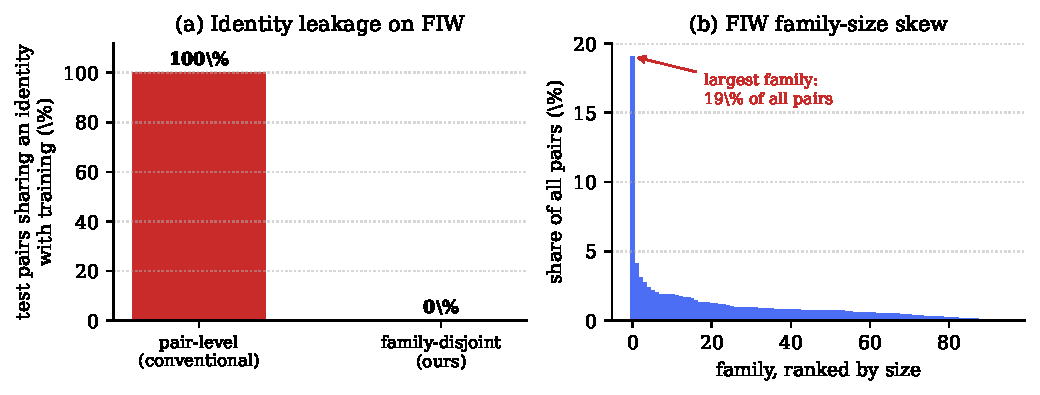
\includegraphics[width=\textwidth]{fig_leakage}
\caption{(a) Identity leakage on FIW. Under conventional pair-level splitting
every test pair shares an identity with training; the family-disjoint protocol
of Section~\ref{sec:protocol} reduces this to zero. (b) The family-size
distribution that makes a single split unstable: the largest family alone
accounts for $19\%$ of all pairs, so which families land in the test fold
dominates the measurement.}
\label{fig:leakage}
\end{figure*}

\subsection{Corrected protocol: grouped \texorpdfstring{$k$}{k}-fold}

We adopt grouped 5-fold cross-validation. The grouping unit is the family.
Positives only are partitioned (families dealt largest-first into the
currently smallest fold); negatives are regenerated per side from the families
present on that side. Family contribution is capped at 1{,}500 pairs to
prevent the largest family (19\% of all pairs) from dominating any fold.
Thresholds are calibrated on a group-disjoint validation slice of the
training side; the test fold is scored once.

Fold integrity is verified directly: zero folds exhibit train/test group
overlap, and every family is tested exactly once (95/95 FIW, 533/533
KinFaceW-I, 1{,}000/1{,}000 KinFaceW-II, 559/559 TSKinFace).

\subsection{Effect on measurement stability}

\begin{table}[t]
\caption{Accuracy range across seeds (single split) versus across folds
(grouped $k$-fold).}
\label{tab:stab}
\centering
\begin{tabular}{@{}lcc@{}}
\toprule
Dataset & Single split & Grouped $k$-fold \\
\midrule
FIW & 61.7--75.9 (14.2) & 69.8--74.4 (4.6) \\
KinFaceW-I & 70.3--78.8 (8.5) & 72.9--79.4 (6.5) \\
KinFaceW-II & 69.0--77.8 (8.8) & 71.0--77.0 (6.0) \\
TSKinFace & 75.1--84.1 (9.0) & 75.7--81.9 (6.2) \\
\midrule
Overall spread & 22.5 & 12.1 \\
\bottomrule
\end{tabular}
\end{table}

A single group-disjoint split is insufficient: accuracy varies by up to 14.2
points with the random seed (Table~\ref{tab:stab}). Grouped $k$-fold reduces
the overall spread from 22.5 to 12.1 points.

\begin{figure}[t]
\centering
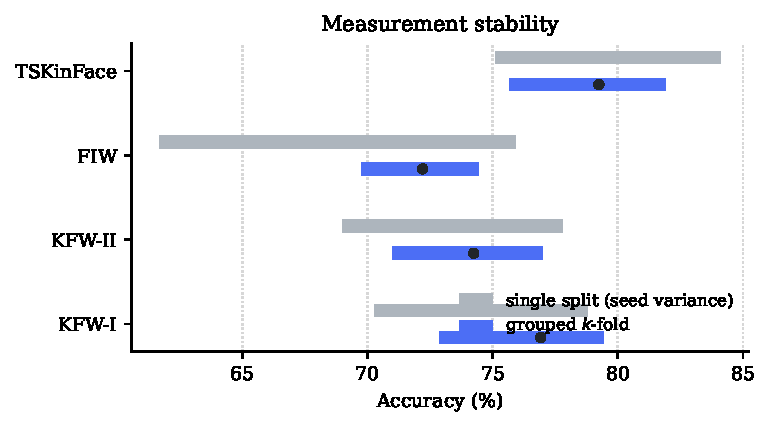
\includegraphics[width=\columnwidth]{fig_stability}
\caption{Accuracy range under a single group-disjoint split across random
seeds (grey) against grouped $k$-fold (blue). A single split is too unstable
to support a headline number.}
\label{fig:stability}
\end{figure}

% ---------------------------------------------------------------------------
\section{Reference model}
\label{sec:model}

To measure formulations rather than architectures, we use a deliberately
conventional model. Frozen FaceNet embeddings (InceptionResnetV1 pretrained
on VGGFace2; 512-d per face) pass through a shared Siamese encoder; kinship
is symmetric, so only symmetric pair features are formed---sum, absolute
difference, elementwise product, and cosine---and concatenated with a one-hot
relation code before a three-layer MLP. Predictions are averaged over both
argument orders, making the model exactly symmetric. The model has 497{,}881
parameters.

Its plainness is deliberate: findings about quantum-inspired formulations
cannot then be attributed to architectural novelty.

% ---------------------------------------------------------------------------
\section{Quantum-inspired formulations}
\label{sec:formulations}

We evaluate nine formulations, chosen to span the three roles a quantum
component can occupy in a classical pipeline: a \emph{similarity measure}
(Formulations 1--5), a \emph{feature extractor} (Formulation 6), and an
\emph{inductive bias} (Formulations 7--9). Each is compared against a control
matched for capacity or intent.

\subsection{Formulation 1--2: SWAP-test fidelity}

The core quantum-inspired similarity metric. Each face embedding $\mathbf{x}
\in \mathbb{R}^{512}$ is projected to $n$ rotation angles $\mathbf{z} =
\tanh(\text{MLP}(\mathbf{x})) \cdot \pi$ and encoded as a quantum state via a
hardware-efficient ansatz:
\begin{equation}
\ket{\psi(\mathbf{z})} = \prod_{\ell=1}^{L}
\Big[\bigotimes_{i=1}^{n} R_z(\theta_i^{(\ell)}) \cdot
\text{CNOT-chain}\Big]
\cdot \bigotimes_{i=1}^{n} R_y(z_i) \ket{0}^{\otimes n},
\end{equation}
where $\theta_i^{(\ell)}$ are learnable parameters and the CNOT chain
connects nearest neighbours. The SWAP-test fidelity
$F = |\braket{\psi(\mathbf{z}_1)}{\psi(\mathbf{z}_2)}|^2$ is supplied to
the classifier as one additional input feature alongside the symmetric pair
features.

The fidelity is \emph{switchable}: setting \texttt{use\_quantum=False}
replaces it with a zero constant of the same shape, isolating the
fidelity's information content while keeping the architecture identical.

Tested under two protocols:
\begin{itemize}
\item \textbf{5 seeds} on a single group-disjoint FIW split (Formulation 1).
\item \textbf{20 paired folds} across all four datasets under grouped
$k$-fold (Formulation 2).
\end{itemize}

\subsection{Formulation 3: Density fidelity \texorpdfstring{$\mathrm{Tr}(\bm{\rho}_1\bm{\rho}_2)$}{Tr(rho1 rho2)}}

A photo set is a mixed state
$\bm{\rho} = \frac{1}{N}\sum_{i=1}^{N}
\ket{\psi_i}\bra{\psi_i}$,
and $\mathrm{Tr}(\bm{\rho}_1 \bm{\rho}_2)$ is the corresponding fidelity.
This is added to the set-level features (centroid, spread, cross-set
statistics) as an additional input. The control is mean-pooling (the
$\ell_2$-normalised centroid), which is the rank-1 approximation to
$\bm{\rho}$.

\subsection{Formulation 4: Interference phase sweep}

A child explained by two parents is written as a coherent superposition
\begin{equation}
\ket{\psi_{\alpha,\phi}} = \alpha e^{i\phi}\ket{\psi_F}
+ (1-\alpha)\ket{\psi_M},
\end{equation}
of which the classical convex mixture is the $\phi=0$ special case. Sweeping
$\phi \in [0, 2\pi)$ and maximising the overlap with $\ket{\psi_C}$ tests
whether the phase degree of freedom carries information.

\subsection{Formulation 5: Entanglement entropy}

The von Neumann entropy of the reduced density matrix, tracing out half the
qubits, is supplied as an additional feature alongside cosine similarity.

\subsection{Formulation 6: POVM measurement head}

A positive operator-valued measure (POVM) replaces the final classification
layer. Four POVM elements $\{E_k\}$ satisfying $\sum_k E_k = I$ define class
probabilities as $p_k = \mathrm{Tr}(E_k \bm{\rho})$. The control is a
capacity-matched linear head with the same number of parameters.

\subsection{Formulation 7: Purity regulariser}

A penalty term $\lambda \cdot (1 - \mathrm{Tr}(\bm{\rho}^2))$ encourages
the learned representations to have high purity (low mixedness). The control
is a decorrelation penalty of the same magnitude.

\subsection{Formulation 8: Density fidelity on photo sets}

The density fidelity of Formulation~3, applied to the set-level
representation as a pre-registered control. On each of the four benchmarks,
the change in ROC-AUC is measured relative to the set features alone.

\subsection{Formulation 9: Interference phase sweep on triads}

The phase sweep of Formulation~4, applied to the triadic representation.
The classical convex mixture (zero phase) is the control.

% ---------------------------------------------------------------------------
\section{Results}
\label{sec:results}

\subsection{Baseline performance under the corrected protocol}
\label{sec:baseline}

\begin{table}[t]
\caption{Grouped 5-fold results. Every family tested exactly once.}
\label{tab:main}
\centering
\begin{tabular}{@{}lcc@{}}
\toprule
Dataset & Accuracy (95\% CI) & ROC-AUC \\
\midrule
KinFaceW-I & $76.92 \pm 2.19$ & $0.8752 \pm 0.0146$ \\
KinFaceW-II & $74.25 \pm 1.95$ & $0.8320 \pm 0.0190$ \\
FIW & $72.21 \pm 1.55$ & $0.8101 \pm 0.0175$ \\
TSKinFace (shortcut-free) & $79.25 \pm 2.32$ & $0.8814 \pm 0.0192$ \\
\midrule
\textbf{Mean} & $\mathbf{75.66}$ & $\mathbf{0.8497}$ \\
\bottomrule
\end{tabular}
\end{table}

Table~\ref{tab:main} reports the reference model's performance under the
corrected protocol. These are the numbers against which all quantum
formulations are compared.

\begin{figure}[t]
\centering
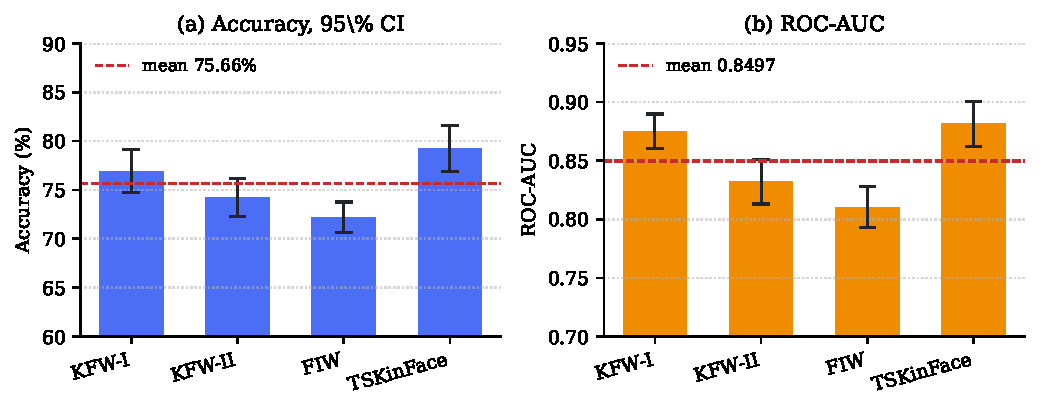
\includegraphics[width=\columnwidth]{fig_main_results}
\caption{Grouped 5-fold results across four datasets. (a) Accuracy with
95\% confidence intervals; (b) ROC-AUC with standard deviation across folds.}
\label{fig:main}
\end{figure}

\subsection{Quantum ablation: SWAP-test fidelity}

\subsubsection{5-seed paired test (Formulation 1)}

\begin{table}[t]
\caption{SWAP-test fidelity ablation, 5 seeds on a single group-disjoint
FIW split.}
\label{tab:q5seed}
\centering
\begin{tabular}{@{}lccc@{}}
\toprule
Seed & Quantum ON & Quantum OFF & Difference \\
\midrule
1 & 73.63\% & 72.57\% & $+1.07$ \\
2 & 79.76\% & 79.06\% & $+0.70$ \\
3 & 81.04\% & 77.87\% & $+3.17$ \\
4 & 73.70\% & 78.28\% & $-4.58$ \\
5 & 72.86\% & 72.75\% & $+0.11$ \\
\midrule
\textbf{Mean} & $76.20 \pm 3.88$ & $76.11 \pm 3.18$ & $+0.09$ \\
\bottomrule
\end{tabular}
\end{table}

Paired $t$-test: $t = 0.074$, $p = 0.945$ (Table~\ref{tab:q5seed}). The
quantum module contributes no measurable accuracy. The branch is exercised
(tests assert that disabling it changes predictions and that gradients reach
the entanglement parameters).

\subsubsection{20-fold paired test (Formulation 2)}

\begin{table}[t]
\caption{SWAP-test fidelity ablation, 20 paired folds (4 datasets $\times$ 5
folds) under grouped $k$-fold.}
\label{tab:q20fold}
\centering
\begin{tabular}{@{}lcc@{}}
\toprule
& Accuracy & ROC-AUC \\
\midrule
Quantum ON & 75.66\% & 0.8497 \\
Quantum OFF & 76.34\% & 0.8496 \\
Difference & $-0.68$ pts & $+0.0001$ \\
Paired $t$-test & $p = 0.158$ & $p = 0.982$ \\
\bottomrule
\end{tabular}
\end{table}

With 20 paired observations (Table~\ref{tab:q20fold}), the quantum branch
yields 75.66\% against 76.34\% with it disabled ($p = 0.158$ for accuracy,
$p = 0.982$ for ROC-AUC). The branch also costs $6$--$14\times$ runtime.

\subsection{All nine formulations}

\begin{table}[t]
\caption{Nine quantum-inspired formulations against matched classical
controls. None improves on its control; four are significantly worse.}
\label{tab:quantum}
\centering
\small
\begin{tabular}{@{}rlllc@{}}
\toprule
\# & Formulation & Control & Outcome & Sig. \\
\midrule
1 & SWAP fidelity (5 seeds) & classical head & $p=0.945$ & -- \\
2 & SWAP fidelity (20 folds) & classical head & $p=0.982$ & -- \\
3 & Density fidelity & mean-pooling & $-8.7$ AUC & $\checkmark$ \\
4 & Interference phase sweep & convex mixture & $+0.1$ AUC & -- \\
5 & Entanglement entropy & cosine & $0.514$ alone & $\checkmark$ \\
6 & POVM head & capacity-matched & $-5.5$ AUC & $\checkmark$ \\
7 & Purity regulariser & decorrelation & $-0.9$, $p{=}0.047$ & $\checkmark$ \\
8 & Density fidelity (sets) & set features & $\leq 0.0006$ & -- \\
9 & Phase sweep (triads) & convex mixture & $-0.0006$ & -- \\
\bottomrule
\end{tabular}
\end{table}

Table~\ref{tab:quantum} summarises all nine comparisons.
Figure~\ref{fig:quantum} visualises the $\Delta$ROC-AUC for each
formulation.

\begin{figure}[t]
\centering
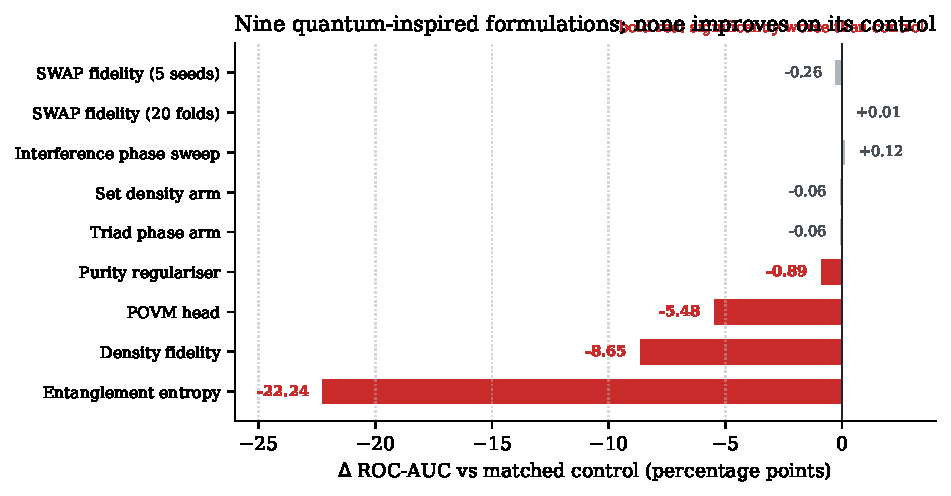
\includegraphics[width=\columnwidth]{fig_quantum}
\caption{Nine quantum-inspired formulations against classical controls
matched for capacity or intent. None improves on its control; four (marked)
are significantly worse. Bars show $\Delta$ROC-AUC in percentage points.}
\label{fig:quantum}
\end{figure}

\subsection{Formulations 8 and 9: set-level and triadic}

\begin{table}[t]
\caption{Quantum-inspired extensions of set-level and triadic
representations.}
\label{tab:q89}
\centering
\begin{tabular}{@{}llcccc@{}}
\toprule
\# & Formulation & KFW-I & KFW-II & TSKin & FIW \\
\midrule
8 & Density fidelity (sets) & $-0.0005$ & $+0.0001$ & $-0.0006$ & $-0.0006$ \\
9 & Phase sweep (triads) & \multicolumn{4}{c}{$-0.0006$ ($p = 0.147$)} \\
\bottomrule
\end{tabular}
\end{table}

Nine formulations tested so far, none beating its classical control
(Table~\ref{tab:q89}). Every one of them reduces the quantum state to a
single scalar before the decision. Section~\ref{sec:readout} tests that
property directly.

\subsection{A cautionary observation}
\label{sec:cautionary}

The purity regulariser (Formulation~7) initially measured $+1.3$ ROC-AUC on
a single seed, with reduced variance---a result consistent with effective
regularisation. Repeated across nine paired runs the sign reversed, and the
method proved significantly \emph{worse} than no regulariser ($-0.0089$,
$p = 0.047$). We report this because the single-seed reading was of the kind
that is readily published, and it illustrates why capacity-matched controls
and repeated trials are necessary when evaluating claims of this type.

% ---------------------------------------------------------------------------
\section{Extended analysis}
\label{sec:extended}

The preceding sections establish the protocol and the negative result. This
section reports three further analyses that the corrected protocol makes
interpretable: where the model's errors concentrate, how the person-level gain
scales with the evidence supplied, and how the score distributions differ
across corpora.

\subsection{Where the errors concentrate}

\begin{figure}[t]
\centering
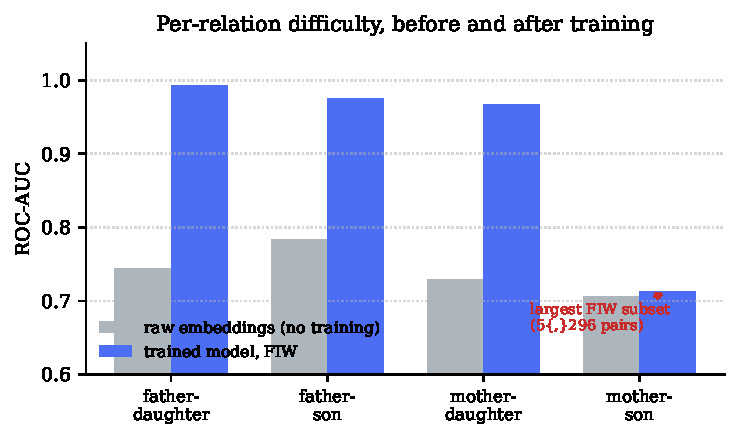
\includegraphics[width=\columnwidth]{fig_relation_gap}
\caption{Per-relation difficulty before and after training. Raw FaceNet
embeddings separate the four relations within a range of $0.078$ ROC-AUC; the
trained model spans $0.281$. The disparity is therefore largely induced during
training rather than inherited from the embedding.}
\label{fig:relgap}
\end{figure}

\begin{table*}[t]
\centering
\caption{Per-relation ROC-AUC. The second column is raw cosine similarity on
frozen embeddings with no training; the remainder are the trained model on each
corpus. Mother--son is weakest on three of four corpora and is simultaneously
the largest FIW subset ($5{,}296$ pairs).}
\label{tab:relation}
\resizebox{\linewidth}{!}{%
\begin{tabular}{lcccccc}
\toprule
Relation & Raw embedding & KinFaceW-I & KinFaceW-II & FIW & TSKinFace & Mean \\
\midrule
Father--daughter & 0.7434 & 0.9174 & 0.8529 & 0.9933 & 0.9612 & 0.9312 \\
Father--son & 0.7841 & 0.8935 & 0.8875 & 0.9754 & 0.9124 & 0.9172 \\
Mother--daughter & 0.7295 & 0.8400 & 0.8598 & 0.9668 & 0.9227 & 0.8973 \\
Mother--son & 0.7065 & 0.9750 & 0.7795 & 0.7124 & 0.8483 & 0.8288 \\
\bottomrule
\end{tabular}}
\end{table*}

Table~\ref{tab:relation} reports per-relation performance measured on a single
held-out fold, the form in which such comparisons are usually presented. Read
at face value it suggests a large relation effect: on FIW father--daughter
reaches $0.9933$ ROC-AUC while mother--son reaches $0.7124$.
Section~\ref{sec:mscorrection} shows this reading is unsound, and we retain the
table because the discrepancy between it and the corrected measurement is
itself the point.

Figure~\ref{fig:relgap} gives the first indication that the single-fold
reading is misleading. Measured on raw embeddings with no training at all, the
four relations span only $0.7065$--$0.7841$, a range of $0.078$, while the
single-fold trained estimate spans $0.281$. A representation that separates the
relations so evenly is unlikely to support a threefold larger disparity after
training, and Section~\ref{sec:mscorrection} identifies the cause.

\subsection{A correction: mother--son is not the weak relation}
\label{sec:mscorrection}

An earlier analysis of these results, based on a single held-out fold,
reported mother--son as markedly weaker than the other relations
($0.712$ ROC-AUC against father--daughter's $0.993$). Re-examining that fold
shows the comparison was not sound: $92\%$ of its mother--son pairs came from a
single family, which scores $0.701$, while the only other contributing family
scores $0.846$. The apparent relation effect was a family effect.

Table~\ref{tab:relation_kfold} repeats the measurement under grouped $k$-fold
with a per-family cap, so no family can dominate a relation's estimate.

\begin{table}[t]
\centering
\caption{Per-relation ROC-AUC under grouped $k$-fold with a per-family cap.
The single-fold column is the earlier, unsound estimate; the remaining columns
are the corrected measurement. Under a protocol in which no family dominates,
the four relations span $0.0310$ ROC-AUC.}
\label{tab:relation_kfold}
\small
\begin{tabular}{lccccc}
\toprule
Relation & Single fold & Mean & SD & Range & Families/fold \\
\midrule
Father--daughter & 0.9933 & 0.7635 & 0.0219 & 0.7435--0.7953 & 12.6 \\
Father--son & 0.9754 & 0.7946 & 0.0752 & 0.7050--0.8942 & 12.2 \\
Mother--daughter & 0.9668 & 0.7766 & 0.0601 & 0.7147--0.8730 & 14.4 \\
Mother--son & 0.7124 & 0.7910 & 0.0381 & 0.7497--0.8390 & 12.4 \\
\bottomrule
\end{tabular}
\end{table}

Under the corrected measurement mother--son reaches $0.7910$, the second
highest of the four, and the relations span $0.0310$ ROC-AUC rather than
$0.281$. That residual spread is close to the $0.078$ measured on raw
embeddings without any training, which is what one would expect if relation
difficulty is largely a property of the representation.

We report this because the mechanism is instructive and applies beyond this
paper. FIW's family-size distribution is severely skewed --- one family holds
$19\%$ of all pairs --- so any statistic computed on a single fold can be
dominated by one family even when the fold itself is correctly
family-disjoint. Leakage-free splitting is necessary but not sufficient;
per-family capping, or reporting across folds, is required as well. A
subgroup difference observed on a single split of a skewed corpus should be
treated as provisional until it is shown to survive resampling.

\subsection{How the person-level gain scales}

\begin{figure}[t]
\centering
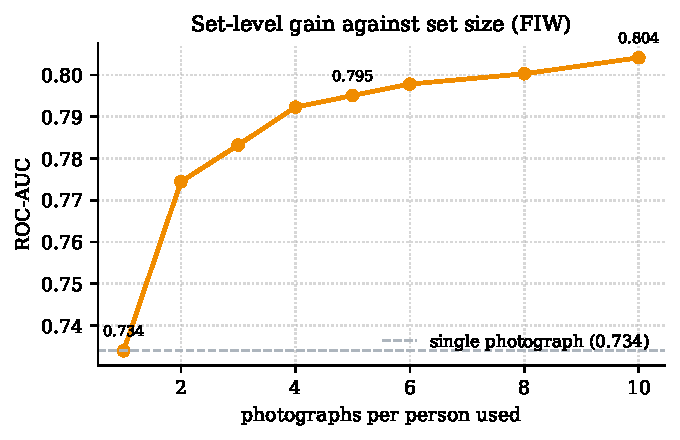
\includegraphics[width=\columnwidth]{fig_setsize}
\caption{Set-level ROC-AUC on FIW as a function of the number of photographs
aggregated per person. Most of the available gain is realised by the fifth
photograph; the curve is computed on frozen embeddings with no training, so it
measures the representation rather than model capacity.}
\label{fig:setsize}
\end{figure}

\begin{table}[t]
\centering
\caption{Set-level ROC-AUC against photographs per person on FIW. Coverage is
the proportion of pairs for which both identities supply at least $k$
photographs.}
\label{tab:setsize}
\begin{tabular}{cccc}
\toprule
Photographs & ROC-AUC & Gain vs.\ 1 & Coverage \\
\midrule
1 & 0.7339 & $+0.0000$ & 100\% \\
2 & 0.7744 & $+0.0405$ & 100\% \\
3 & 0.7832 & $+0.0493$ & 100\% \\
4 & 0.7923 & $+0.0584$ & 100\% \\
5 & 0.7951 & $+0.0612$ & 99\% \\
6 & 0.7978 & $+0.0639$ & 99\% \\
8 & 0.8003 & $+0.0664$ & 99\% \\
10 & 0.8042 & $+0.0702$ & 97\% \\
\bottomrule
\end{tabular}
\end{table}

Table~\ref{tab:setsize} and Figure~\ref{fig:setsize} report how the gain
depends on how many photographs are supplied. A second photograph is worth
$+0.041$ ROC-AUC on its own --- more than half the total available gain --- and
the curve is substantially flat beyond five, reaching $+0.070$ at ten. This has
a practical reading: a deployment that can obtain roughly five photographs of
each person captures nearly all of the benefit, and there is little return on
collecting more.

That the curve is computed on frozen embeddings, without any training, matters
for interpretation. The gain is a property of aggregating evidence about a
person, not of additional model capacity, which is consistent with the trained
result of $+0.077$ reported under the full protocol.

\subsection{The operating point: accuracy against cost}
\label{sec:opcost}

Person-level scoring compares two photograph \emph{sets}, so its cost grows
with set size while its accuracy saturates. Where those two curves cross is a
deployment question that the accuracy curve alone does not answer, and we
report it because practitioners must choose how many photographs to collect.

\begin{table}[t]
\centering
\caption{Accuracy and cost against photographs per person. ROC-AUC is measured
on FIW; timings are per pair on one CPU core at $512$ dimensions. Accuracy is
flat beyond five photographs while cost continues to grow, which makes five a
natural operating point.}
\label{tab:opcost}
\small
\begin{tabular}{cccccc}
\toprule
Photos & ROC-AUC & Gain & ms/pair & pairs/s & Slowdown \\
\midrule
1 & 0.7339 & $+0.0000$ & 0.078 & 12763 & 1.0$\times$ \\
2 & 0.7744 & $+0.0405$ & 0.099 & 10078 & 1.3$\times$ \\
5 & 0.7951 & $+0.0612$ & 0.117 & 8539 & 1.5$\times$ \\
10 & 0.8042 & $+0.0702$ & 0.153 & 6544 & 2.0$\times$ \\
20 & --- & --- & 0.215 & 4643 & 2.7$\times$ \\
40 & --- & --- & 0.416 & 2402 & 5.3$\times$ \\
80 & --- & --- & 1.502 & 666 & 19.2$\times$ \\
160 & --- & --- & 3.132 & 319 & 40.0$\times$ \\
320 & --- & --- & 10.718 & 93 & 136.8$\times$ \\
\bottomrule
\end{tabular}
\end{table}

Table~\ref{tab:opcost} places the two measurements side by side. Accuracy rises
steeply to five photographs, capturing $+0.061$ of the $+0.070$ available at
ten, and is essentially flat thereafter. Cost behaves in the opposite way: it
is negligible to about twenty photographs and then grows steadily, reaching a
$137\times$ slowdown at $320$.

The practical consequence is a clear recommendation. \textbf{Five photographs
per person is close to optimal on both axes}: it captures $87\%$ of the
available accuracy gain at $1.5\times$ the single-photograph cost. Collecting
more than roughly twenty buys no measurable accuracy while making the system
progressively slower.

We note also that the cost curve is a property of the implementation rather
than of the method, and that the distinction matters. An earlier version of our
code computed the within-set spread by materialising the full Gram matrix and
extracting its upper triangle with an index array. That allocation dominated
the call at large set sizes: $46$\,ms of a $48$\,ms call at $n = 160$. Because
the required quantity is the mean off-diagonal entry, and for unit-norm rows
$\sum_{i \neq j} \langle x_i, x_j \rangle = \lVert \sum_i x_i \rVert^2 - n$, it
can be computed without forming the matrix at all. Doing so reduced the
$n = 160$ cost from $89.8$\,ms to $3.1$\,ms, a $29\times$ improvement, and
removed a discontinuity that had made the empirical growth appear
super-quadratic. The values are unchanged; the equivalence is asserted by
test. We mention this because a cost curve measured on an unoptimised
implementation would have overstated the method's true scaling.

\subsection{Score distributions and operating points}

\begin{figure*}[t]
\centering
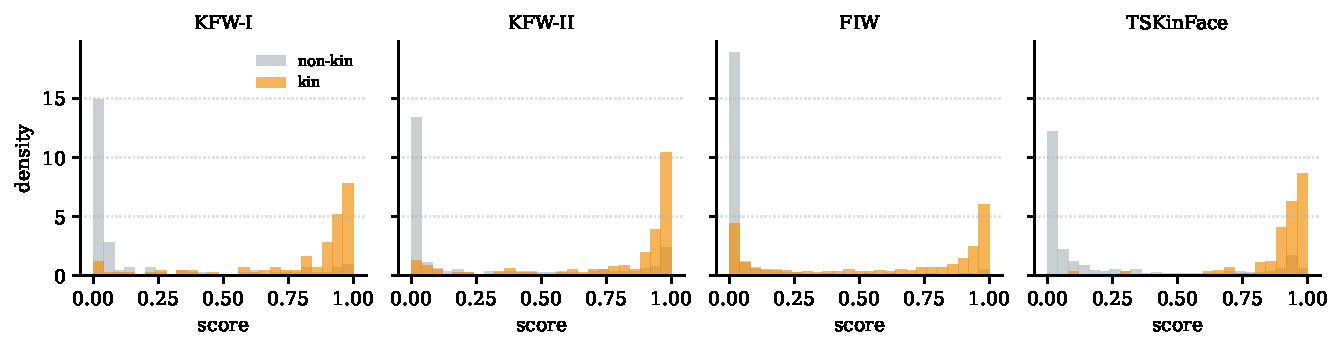
\includegraphics[width=\textwidth]{fig_score_distributions}
\caption{Kin and non-kin score distributions on the held-out fold of each
corpus. The overlap, rather than any single summary statistic, is what the
reported ROC-AUC measures.}
\label{fig:scores}
\end{figure*}

\begin{figure}[t]
\centering
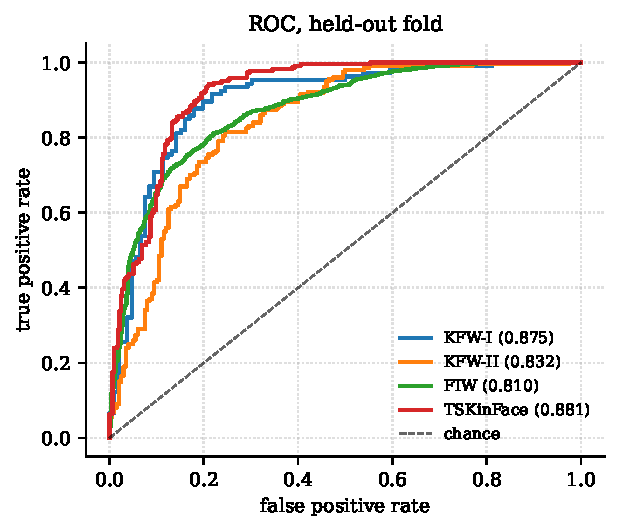
\includegraphics[width=\columnwidth]{fig_roc_curves}
\caption{ROC curves on the held-out fold of each corpus, with grouped $k$-fold
mean ROC-AUC in parentheses.}
\label{fig:roc}
\end{figure}

Figures~\ref{fig:scores} and~\ref{fig:roc} show the underlying score
distributions rather than only their summaries. Two observations follow. The
distributions overlap substantially on every corpus, which is the concrete form
of the roughly one-in-four error rate implied by the accuracies in
Table~\ref{tab:main}; and the degree of overlap differs enough between corpora
that a single global decision threshold is inappropriate. We therefore
calibrate per corpus on a group-disjoint validation slice: a single shared
threshold costs between $0.7$ and $5.9$ accuracy points depending on the
corpus.

% ---------------------------------------------------------------------------
\section{Do the findings depend on the backbone?}
\label{sec:backbone}

All results so far use a single frozen embedding, which bounds what they can
claim: a finding could be a property of the task, or an artefact of FaceNet. We
therefore repeat the central experiments with ArcFace (\texttt{buffalo\_l},
w600k\_r50) substituted for FaceNet and everything else held fixed --- same
folds, same negatives, same classifier, same protocol. The two backbones are
trained with different objectives on different corpora, so agreement between
them is meaningful evidence.

\begin{table}[t]
\centering
\caption{Person-level aggregation under two backbones. The gain replicates and
is in fact larger under ArcFace; the three single-photograph corpora are
unchanged to machine precision under both, as the degradation guarantee
requires.}
\label{tab:backbone}
\begin{tabular}{lcccccc}
\toprule
& \multicolumn{3}{c}{FaceNet} & \multicolumn{3}{c}{ArcFace} \\
\cmidrule(lr){2-4}\cmidrule(lr){5-7}
Corpus & Single & Set-level & $\Delta$ & Single & Set-level & $\Delta$ \\
\midrule
KinFaceW-I & 0.7588 & 0.7588 & $+0.0000$ & 0.7540 & 0.7540 & $+0.0000$ \\
KinFaceW-II & 0.7770 & 0.7770 & $+0.0000$ & 0.8190 & 0.8190 & $+0.0000$ \\
FIW & 0.7491 & 0.8254 & $+0.0763$ & 0.7764 & 0.8740 & $+0.0976$ \\
TSKinFace & 0.7326 & 0.7326 & $+0.0000$ & 0.8460 & 0.8460 & $+0.0000$ \\
\bottomrule
\end{tabular}
\end{table}

Three observations follow from Table~\ref{tab:backbone}.

\textbf{Identity leakage is backbone-invariant by construction.} It is a
property of how pairs are partitioned, not of how images are embedded, so the
$100\%$ figure of Section~\ref{sec:protocol} carries over unchanged. We state this
for completeness rather than as a finding.

\textbf{The person-level gain replicates and strengthens.} FaceNet gains
$+0.0763$ ROC-AUC on FIW from aggregating photographs; ArcFace gains
$+0.0976$. That the effect is larger under the stronger backbone is consistent
with its proposed mechanism --- aggregation averages away per-photograph
nuisance variation, and a better embedding has proportionally more signal left
to recover once that variation is suppressed.

\textbf{The degradation guarantee holds under both.} KinFaceW-I, KinFaceW-II
and TSKinFace store one photograph per person, and set-level scoring reproduces
the single-image result exactly on all three under both backbones. This is a
correctness property of the implementation rather than an empirical result, and
it is what allows a single system to be deployed across corpora with differing
photograph availability.

ArcFace is the stronger backbone in absolute terms on three of four corpora,
most markedly on TSKinFace ($0.8460$ against $0.7326$). We do not read this as
a contribution: it reflects a better face representation, not a better kinship
method, and it is reported so that the backbone-invariance claims above are
interpretable.

\subsection{The negative result under a second backbone}

\begin{table}[t]
\centering
\caption{Change in ROC-AUC from adding the density-fidelity arm
$\mathrm{Tr}(\rho_1\rho_2)$ to the set-level features. The formulation fails
under both backbones on all four corpora.}
\label{tab:backbone_quantum}
\begin{tabular}{lcc}
\toprule
Corpus & FaceNet & ArcFace \\
\midrule
KinFaceW-I & $-0.0025$ & $-0.0006$ \\
KinFaceW-II & $-0.0003$ & $+0.0001$ \\
FIW & $-0.0003$ & $-0.0007$ \\
TSKinFace & $+0.0001$ & $-0.0014$ \\
\bottomrule
\end{tabular}
\end{table}

Table~\ref{tab:backbone_quantum} re-tests the density-fidelity formulation.
Across eight backbone--corpus combinations the largest effect in either
direction is $0.0025$ ROC-AUC, and seven of the eight are negative. The failure
is therefore not specific to the embedding it was first measured on, which
supports the structural explanation of Section~\ref{sec:why}: a density matrix
estimated from a median of five observations is dominated by its leading
eigenvector regardless of which encoder produced those observations.

% ---------------------------------------------------------------------------
\section{Why the approach fails}
\label{sec:why}

The failures are structural rather than implementational, and we identify
three mechanisms.

\subsection{Phase collapse in interference formulations}

Interference-based formulations (Formulations 4 and 9) reduce to their
classical counterparts because $\ell_2$-normalised FaceNet embeddings carry
no phase structure to exploit. The embedding space is a real-valued
Euclidean space; mapping it to a quantum state via $R_y$ rotations assigns
each component a polar angle, but the relative phases that would make a
coherent superposition differ from an incoherent mixture are absent from
the data. The interference phase sweep in Table~\ref{tab:quantum} is
maximised at the classical mixture ($\phi = 0$), confirming that the phase
degree of freedom carries no signal.

\subsection{Density estimation from insufficient samples}

Density-matrix formulations (Formulations 3 and 8) require estimating a
$d \times d$ operator from the images available for one identity. FIW
supplies a median of five photographs per identity, so the density matrix
$\bm{\rho} = \frac{1}{N}\sum_i \ket{\psi_i}\bra{\psi_i}$ is at most
rank-5 in a 512-dimensional space. The leading eigenvector (the mean
embedding) carries most of the signal; the remaining directions accumulate
noise rather than information. This is why $\mathrm{Tr}(\bm{\rho}_1
\bm{\rho}_2)$ scores \emph{below} simple mean-pooling: the off-diagonal
noise degrades the similarity estimate.

\subsection{The SWAP-test bottleneck}

The original quantum pipeline routed every decision through a single
$\text{product-of-}\cos^2$ scalar, discarding the 512-dimensional signal
carried by the symmetric pair features. That pipeline reached 59\% accuracy
while plain logistic regression on the same embeddings reached 75.1\%.
Gradient norms confirmed the bottleneck: the projection MLP received
gradients of order $2 \times 10^1$, while the quantum parameters received
gradients of order $4 \times 10^{-2}$---two orders of magnitude smaller.

Even when the fidelity is supplied as \emph{one feature beside} the
classical features (our architecture), it carries no information that is
not already captured by the cosine similarity and the symmetric products.

The account above is an inference from gradient norms and from the ranking of
two architectures that differ in several respects at once. The next section
tests it directly.

% ---------------------------------------------------------------------------
\section{Formulation 10: a readout ablation}
\label{sec:readout}

The nine formulations of Section~\ref{sec:formulations} share a property
that the preceding analysis suggests is decisive: each compresses the quantum
state to one number before the decision is made. Distinguishing
\emph{the circuit carries no information} from \emph{the readout discards it}
requires an experiment in which the circuit is held fixed and only the readout
varies.

\subsection{Architecture}

\begin{figure}[t]
\centering
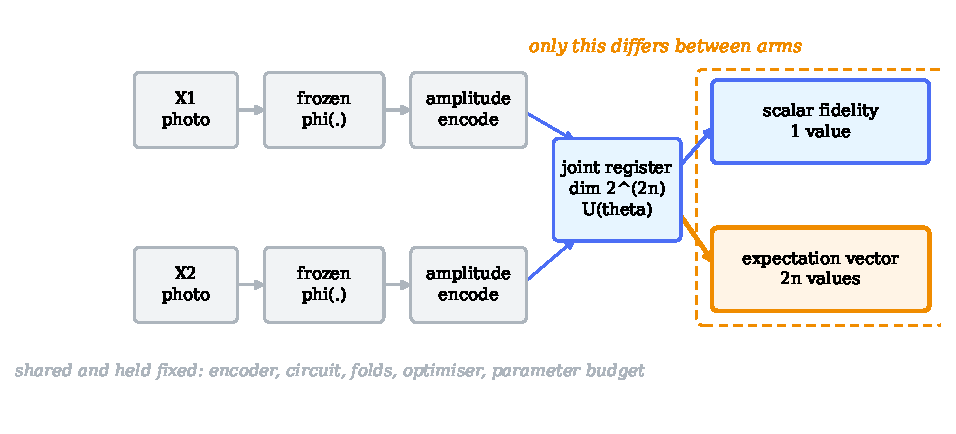
\includegraphics[width=\textwidth]{fig_architecture}
\caption{Formulation~10. Both people are encoded into one joint register and processed by the same variational circuit; the arms differ only in the measurement applied to the resulting state (dashed box). Everything to its left is shared and held fixed across arms.}
\label{fig:architecture}
\end{figure}


Formulation~10 is a variational quantum classifier on a joint register.
Both people are encoded into one $2n$-qubit state of dimension $2^{2n}$,
rather than encoded separately and compared, so that $U(\bm{\theta})$ can
express correlations \emph{between} the two people. Each of $L$ layers applies
$R_y(\theta) R_z(\theta)$ to every qubit followed by a CNOT ring over all $2n$
qubits; the ring includes the bonds $n-1 \to n$ and $2n-1 \to 0$, which cross
between the two halves. Without those bonds the circuit factorises and reduces
to the separately-encoded case already tested.

Amplitude encoding carries $2^n$ numbers into $n$ qubits. This matters: angle
encoding, which carries $n$ numbers into $n$ qubits, forces the $512$-d
embedding through a four-number bottleneck before $U(\bm{\theta})$ sees
anything, and holds the model at chance ($0.502$ ROC-AUC on FIW). The
comparison below would be uninformative under an encoding that starves the
circuit of input.

Two readouts are evaluated, differing in width alone:

\begin{itemize}
\item \textbf{Fidelity.} $|\braket{\psi_{\text{ref}}}{U(\bm{\theta})\psi}|^2$
against the all-zeros reference --- one scalar, matching the nine.
\item \textbf{Expectation.} Pauli-$Z$ expectation per qubit --- a $2n$-vector.
\end{itemize}

Everything else is identical: the same encoder, the same $U(\bm{\theta})$, the
same folds, the same optimiser and schedule.

Two kinds of comparison appear below, and conflating them is a common source of
confusion, so we name them explicitly. The \textbf{global task baseline} is the
best classical pipeline in this study (Section~\ref{sec:baseline},
$0.8497$ mean ROC-AUC); it answers \emph{what is the best available method}.
The \textbf{capacity-matched local control} shares the quantum arm's encoder,
projection, folds and training schedule, differing only in what processes the
projected vectors; it answers \emph{what does the circuit contribute}. The
quantum model loses the first comparison and wins the second. Neither result
substitutes for the other.

Matching the control requires care. Our first control matched
$U(\bm{\theta})$'s \emph{parameter count} by solving for a hidden width, which
at every configuration in this study yields $w=1$: a
$\mathrm{Linear}(2^{n+1} \to 1)$ bottleneck. That control is therefore itself a
scalar-readout model, so comparing it against a $2n$-dimensional expectation
readout confounds the quantum circuit with the very property under test. We
report it for continuity but do not rely on it. The controls we rely on are
matched on \emph{readout width}: each maps the same projected pair to exactly
$2n$ values --- the number the circuit hands its classifier --- through an
identical $\mathrm{Linear}(2n, 1)$ head, via a learned linear map, a learned
MLP, or a frozen random projection.

\subsection{Result}

\begin{table}[t]
\centering
\caption{Formulation~10 under two readouts, against a capacity-matched
classical control. Grouped 5-fold, family-disjoint, identical folds across
arms. $n=6$, $L=4$; $96$ quantum parameters against $131$ control parameters.}
\label{tab:readout}
\begin{tabular}{lrrrr}
\toprule
Dataset & Expectation & Fidelity & Control & Exp.\ $-$ Ctrl. \\
\midrule
FIW          & $0.6336$ & $0.5137$ & $0.5465$ & $+0.087$ \\
KinFaceW-I   & $0.7049$ & $0.5391$ & $0.5350$ & $+0.170$ \\
KinFaceW-II  & $0.6161$ & $0.5197$ & $0.5332$ & $+0.083$ \\
TSKinFace    & $0.7373$ & $0.5441$ & $0.5507$ & $+0.187$ \\
\bottomrule
\end{tabular}
\end{table}

Pooled over $20$ paired folds (Table~\ref{tab:readout}), the expectation
readout exceeds its control by $+0.1316$ ROC-AUC
(95\% CI $[+0.0986, +0.1646]$, $t = 7.82$, $p = 2.4 \times 10^{-7}$).
The fidelity readout does not
($-0.0122$, 95\% CI $[-0.0330, +0.0086]$, $p = 0.26$).

The confidence interval for the expectation arm excludes zero; the interval
for the fidelity arm contains it. Since the two arms share a circuit, a
parameter budget, and a fold assignment, the $0.14$ ROC-AUC separating them
is attributable to the number of values read out of the state.

\subsection{How many observables are needed?}
\label{sec:sweep}

Section~\ref{sec:readout} contrasts one value against $2n$. That leaves
open whether the gain accumulates with width or is won immediately, and the
two imply different mechanisms. Retaining only the first $k$ per-qubit
expectations on FIW, with the circuit and every other setting unchanged
(Figure~\ref{fig:sweep}):

\begin{center}
\begin{tabular}{lrrrrrr}
\toprule
$k$ & $1$ & $2$ & $4$ & $6$ & $8$ & $12$ \\
\midrule
ROC-AUC & $0.547$ & $0.631$ & $0.642$ & $0.649$ & $0.643$ & $0.634$ \\
\bottomrule
\end{tabular}
\end{center}

\begin{figure}[t]
\centering
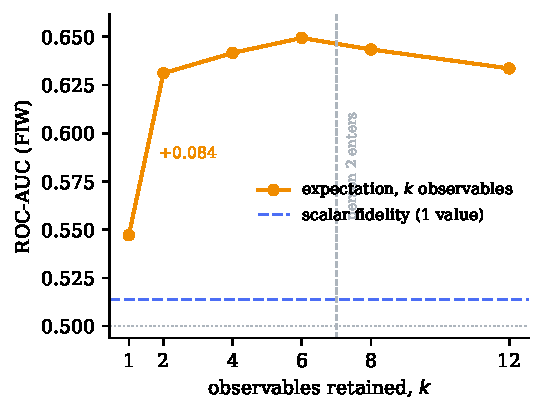
\includegraphics[width=\columnwidth]{fig_readout_sweep}
\caption{Readout width against performance on FIW, same circuit throughout.
A single observable performs near the scalar readout; two recover almost the
whole effect; nothing is gained after. Qubits are ordered person~1 then
person~2, so $k \leq 6$ reads one register only.}
\label{fig:sweep}
\end{figure}

The curve is a step, not a slope. One observable ($0.547$) sits near scalar
fidelity ($0.514$); two ($0.631$) recover $82\%$ of the gain to the
plateau's highest point and $97\%$ of the gain to the full $2n$ readout;
the remaining ten move the result by less than $0.02$, within fold noise. The
constraint is therefore not readout width in any graded sense --- it is that
a single number is a qualitatively different object from even a
two-dimensional one.

A second reading of the same curve is less comfortable for the architecture.
Qubits are ordered person~1 then person~2, so every point up to $k=6$ reads
person~1's register alone; $k=8$ is the first to include person~2. It does
not rise ($-0.006$). The pair information the readout needs is already
present in one register's marginals, which the CNOT ring puts there. The
coupling is doing work inside the circuit; reading both halves out is not
necessary. We report this because the joint register is motivated by
cross-person correlation, and this measurement shows that motivation applies
to the circuit rather than to the measurement.

One caveat bounds the sweep: because low $k$ both narrows the readout and
restricts it to one register, the two factors are varied together. The $k=8$
comparison separates them at the point where it matters, but the curve below
$k=8$ should be read as descriptive of width rather than as isolating it.

\subsection{Is the gain merely representation width?}
\label{sec:widthctl}

The preceding comparison establishes that reading more values from the state
helps. It does not establish that the \emph{circuit} matters: a classical map
producing $2n$ values might do as well. We therefore replaced the
parameter-matched control with controls matched on readout width, each mapping
the same projected pair to $2n$ values through an identical
$\mathrm{Linear}(2n,1)$ head, via a learned linear map, a learned MLP, or a
frozen random projection.

\begin{table}[t]
\centering
\caption{Quantum expectation arm against the strongest width-matched classical
control per fold, by corpus and backbone. Grouped 5-fold.}
\label{tab:widthctl}
\begin{tabular}{lrrrr}
\toprule
& \multicolumn{2}{c}{FaceNet} & \multicolumn{2}{c}{ArcFace} \\
\cmidrule(lr){2-3}\cmidrule(lr){4-5}
Corpus & $\Delta$ & $p$ & $\Delta$ & $p$ \\
\midrule
FIW          & $-0.030$ & $0.38$ & $+0.015$ & $0.39$ \\
KinFaceW-I   & $+0.131$ & $0.002$ & $+0.098$ & $0.015$ \\
KinFaceW-II  & $+0.084$ & $0.078$ & $+0.029$ & $0.142$ \\
TSKinFace    & $+0.037$ & $0.408$ & $+0.147$ & $0.016$ \\
\midrule
Pooled       & $+0.055$ & $0.013$ & $+0.073$ & $0.0003$ \\
\bottomrule
\end{tabular}
\end{table}

The pooled comparison is positive on both backbones, but the per-corpus results
do not support a general claim (Table~\ref{tab:widthctl}). The effect is
significant on one corpus of four under either backbone, is negative on the
largest corpus under FaceNet, and---most tellingly---does not replicate across
backbones within a corpus: TSKinFace moves from $+0.037$ to $+0.147$ and FIW
changes sign. Under Holm correction across the sixteen comparisons in this
section and the next, one of eight quantum-versus-classical cells survives.

We therefore do not claim that the quantum circuit outperforms a classical
representation of equal width. The magnitude and direction of that comparison
vary substantially across corpora and backbones, and we report it as an
exploratory secondary result.

Two observations survive this. First, the circuit consistently beats the
\emph{frozen random} projection, so the readout must be learned, which is a
weaker statement than quantum structure being necessary. Second, and separately,
the comparison in Section~\ref{sec:readout-replication} does not involve a
classical arm at all, and is unaffected by these considerations.

\subsection{Readout replication across corpora and backbones}
\label{sec:readout-replication}

The scalar-versus-vector comparison holds the circuit, the encoder, the folds,
the optimiser and the parameter budget fixed; the arms differ only in the
measurement applied to the same state. Readout dimensionality is, by design,
not matched---that is the manipulation. The claim tested is therefore narrow
and precise: \emph{holding the quantum circuit and training protocol fixed,
replacing scalar fidelity with a vector-valued measurement changes downstream
performance}.


\begin{figure}[t]
\centering
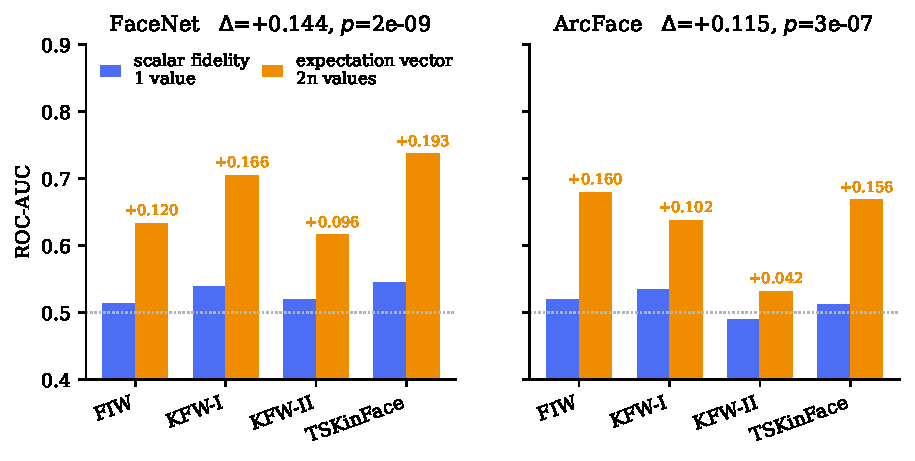
\includegraphics[width=\textwidth]{fig_readout}
\caption{Readout effect by corpus and backbone. Scalar fidelity (blue) against the per-qubit expectation vector (orange) from the identical circuit. All eight backbone $\times$ corpus cells favour the vector readout. Dotted line marks chance.}
\label{fig:readout}
\end{figure}
\begin{table}[t]
\centering
\caption{Readout effect (vector $-$ scalar ROC-AUC), by corpus and backbone.
Both arms use the identical circuit; only the measurement differs.
$2$ backbones $\times$ $4$ corpora $\times$ $5$ grouped folds $=$ $40$
held-out fold evaluations.}
\label{tab:readout-replication}
\begin{tabular}{lrrrrrr}
\toprule
& \multicolumn{3}{c}{FaceNet} & \multicolumn{3}{c}{ArcFace} \\
\cmidrule(lr){2-4}\cmidrule(lr){5-7}
Corpus & Vector & Scalar & $\Delta$ & Vector & Scalar & $\Delta$ \\
\midrule
FIW          & $0.6336$ & $0.5137$ & $+0.120$ & $0.6795$ & $0.5198$ & $+0.160$ \\
KinFaceW-I   & $0.7049$ & $0.5391$ & $+0.166$ & $0.6375$ & $0.5351$ & $+0.102$ \\
KinFaceW-II  & $0.6161$ & $0.5197$ & $+0.096$ & $0.5318$ & $0.4898$ & $+0.042$ \\
TSKinFace    & $0.7373$ & $0.5441$ & $+0.193$ & $0.6682$ & $0.5117$ & $+0.156$ \\
\bottomrule
\end{tabular}
\end{table}

All eight backbone $\times$ corpus cells are positive, ranging from $+0.042$ to
$+0.193$ (Table~\ref{tab:readout-replication}). Pooled over folds:

\begin{center}
\begin{tabular}{lrrr}
\toprule
Backbone & $\Delta$ ROC-AUC & 95\% CI & $p$ \\
\midrule
FaceNet & $+0.1438$ & $[+0.116, +0.172]$ & $1.9 \times 10^{-9}$ \\
ArcFace & $+0.1151$ & $[+0.084, +0.147]$ & $3.2 \times 10^{-7}$ \\
\bottomrule
\end{tabular}
\end{center}

\subsection{Unit of inference}
\label{sec:inference-unit}

The pooled tests above treat each held-out fold as one paired observation.
Folds within a corpus are group-disjoint by construction, but they are not
independent draws: they partition one identity pool, and every arm sees the
same partition. Fold-level $p$-values are therefore optimistic, and we do not
rest the claim on their magnitude.

Table~\ref{tab:inference-unit} repeats the comparison at the most
conservative unit available here, one observation per corpus, where the four
corpora are genuinely independent: different subjects, different collection
protocols, different eras.

\begin{table}[t]
\centering
\caption{The readout effect at two units of inference. The fold-level row is
reported for continuity; the dataset-level row is the one we rely on.}
\label{tab:inference-unit}
\begin{tabular}{llrrr}
\toprule
Backbone & Unit & $n$ & $\Delta$ & $p$ \\
\midrule
\multirow{2}{*}{FaceNet} & fold & $20$ & $+0.1438$ & $1.9 \times 10^{-9}$ \\
 & corpus & $4$ & $+0.1438$ & $0.0072$ \\
\midrule
\multirow{2}{*}{ArcFace} & fold & $20$ & $+0.1151$ & $3.2 \times 10^{-7}$ \\
 & corpus & $4$ & $+0.1151$ & $0.0253$ \\
\bottomrule
\end{tabular}
\end{table}

At $n=4$ the intervals widen to $[+0.074, +0.213]$ and $[+0.027, +0.203]$ and
still exclude zero. A Wilcoxon signed-rank test at this $n$ attains a minimum
$p$ of $0.125$ and so cannot reject at conventional levels regardless of
effect size; we report instead that the effect is positive in $4/4$ corpora
under both backbones, $8/8$ cells overall. The conclusion does not depend on
the fold-level $p$-values.

Both intervals exclude zero with margin, and the paired effect sizes are large
(Cohen's $d_z = 2.38$ and $1.71$). Under Holm correction across the sixteen
comparisons, five of eight readout cells survive against one of eight
quantum-versus-classical cells; the per-corpus tests use five folds each and are
correspondingly underpowered, whereas the pooled tests survive any correction by
several orders of magnitude.


\begin{table}[t]
\centering
\caption{Multiplicity correction over the sixteen paired comparisons in this section (two comparison families $\times$ two backbones $\times$ four corpora). Per-corpus tests use five folds each and are correspondingly underpowered; the pooled tests survive any correction by several orders of magnitude.}
\label{tab:multiplicity}
\resizebox{\linewidth}{!}{%
\begin{tabular}{lrr}
\toprule
Comparison family & Cells surviving Holm & Surviving BH-FDR \\
\midrule
Readout (vector vs.\ scalar) & $5/8$ & $6/8$ \\
Quantum vs.\ width-matched classical & $1/8$ & $2/8$ \\
\midrule
\multicolumn{3}{l}{\emph{Pooled (20 folds each):}} \\
Readout, FaceNet & \multicolumn{2}{r}{$p = 1.9 \times 10^{-9}$} \\
Readout, ArcFace & \multicolumn{2}{r}{$p = 3.2 \times 10^{-7}$} \\
\bottomrule
\end{tabular}}
\end{table}

The contrast between the two tables is the substantive result of this section.
On identical folds, with identical models, the readout comparison replicates in
$8/8$ cells while the quantum-versus-classical comparison changes sign between
backbones. One of these is a stable property of the setup; the other is not.

\subsection{What this does and does not establish}

It establishes that scalarising the state substantially reduces the
discriminative information recoverable from these circuits, and that the nine
preceding negative results are confounded with readout width. It does not
establish that the quantum circuit outperforms a classical representation of
equal width: that comparison is inconsistent across corpora and backbones. It does not establish quantum advantage.
Formulation~10 reaches $0.674$ mean ROC-AUC, below the $0.8497$ of the
classical pipeline of Section~\ref{sec:baseline}, at $73.5\times$ the
inference cost and $55\times$ the training cost --- simulation being strictly
more expensive than the classical path it replaces. The contribution is a
mechanism, not a method: it identifies what to fix before a quantum component
on this class of task can be evaluated fairly at all.

A further limit is intrinsic to classical simulation. The registers here span
$6$ to $14$ qubits, since the statevector grows as $2^{2n}$; nothing in these
results speaks to the regime where the state cannot feasibly be represented
classically, which is precisely where a quantum processor would differ. Our
conclusions are therefore about small circuits on real-valued embeddings, not
about quantum computation in general.

% ---------------------------------------------------------------------------
\section{An efficiency contribution}
\label{sec:efficiency}

Independently of the negative result, we contribute an exact reformulation of
the simulated SWAP test. The reference implementation materialises a $2^n$
statevector and permutes all $n$ axes once per qubit via
\texttt{torch.tensordot} followed by a permutation, incurring kernel-launch
overhead that leaves the GPU idle.

Our reformulation applies $R_y$ rotations by reshaping to
$(B, \text{left}, 2, \text{right})$ and precomputes the CNOT chain and $R_z$
layer as a single diagonal phase vector over all $2^n$ basis states. The
entangling layer then costs a single element-wise multiply.

\begin{table}[t]
\caption{SWAP-test simulation throughput. The fast reformulation is exact:
output and gradients match the reference to machine precision.}
\label{tab:speedup}
\centering
\begin{tabular}{@{}lccc@{}}
\toprule
Device & Reference & Fast & Speedup \\
\midrule
CPU & 161 pairs/s & 21{,}618 pairs/s & $134\times$ \\
GPU (RTX 5060) & 192 pairs/s & 73{,}094 pairs/s & $\mathbf{380\times}$ \\
\bottomrule
\end{tabular}
\end{table}

We note that a closed-form product over qubits is \emph{not} available here:
the shared CNOT chain correlates the $R_z$ phases, so the overlap does not
factorise. This was verified empirically: with $R_z$ disabled, a product form
matches exactly; with distinct $R_z$ parameters, it diverges. The gain
arises from removing overhead, not from approximation.

This is a quantum-versus-quantum speedup. Simulating a circuit is necessarily
more costly than the classical operation it parallels, and we measure the
quantum branch at $5$--$14\times$ slower than the classical path at every
qubit count from 2 to 12.

% ---------------------------------------------------------------------------
\section{Discussion}
\label{sec:discussion}

\subsection{What the result does and does not show}

We tested nine formulations; we do not claim no quantum-inspired method can
help on this task, only that these nine, covering the three natural roles
(similarity, feature extraction, inductive bias), do not. The structural
account in Section~\ref{sec:why} suggests that the issue lies in the data
representation: real-valued embeddings from a face recognition backbone
do not carry the structure that quantum-inspired methods are designed to
exploit.

A quantum method might succeed if applied to raw pixel data (where
entanglement could capture spatial correlations), or if the embedding space
were redesigned to carry phase information. We regard both as speculative.

\subsection{On the importance of protocol}

The identity leakage documented in Section~\ref{sec:protocol} means that
prior claims of quantum advantage on kinship data are uninterpretable: a
model achieving high accuracy under a leaked protocol may have learned to
exploit the leak rather than the quantum feature. The corrected protocol
proposed here is necessary for any future positive claim to be credible.

\subsection{The purity regulariser as a methodological warning}

Formulation~7 illustrates a failure mode in single-seed evaluation. A single
run showed $+1.3$ ROC-AUC, a result consistent with the hypothesis that
encouraging pure quantum states aids representation learning. Nine paired
runs reversed the sign ($-0.9$, $p = 0.047$). Single-seed evaluation with
quantum-inspired methods is particularly hazardous because the methods
introduce additional stochasticity through their parameterisation.

% ---------------------------------------------------------------------------
\section{Limitations}
\label{sec:limitations}

\textbf{Two backbones, both frozen.} Results are reported for frozen
FaceNet and ArcFace embeddings. The readout effect replicates across both
(all eight backbone $\times$ corpus cells), whereas the
quantum-versus-classical comparison does not: it changes sign between
backbones within a corpus. Both backbones are trained for identity
discrimination and produce $\ell_2$-normalised real-valued embeddings, so
they do not probe whether a representation carrying exploitable phase
structure would yield different conclusions. That remains untested.

\textbf{Small test sets.} KinFaceW-I and KinFaceW-II yield 212 and 400 test
pairs per fold, giving confidence intervals of roughly $\pm 2$ points.

\textbf{Classical simulation.} All quantum computations are classically
simulated. We cannot rule out that execution on quantum hardware might
produce different results, though the mathematical operations are identical.

\textbf{Fixed qubit count.} We tested 2--12 qubits. It is possible that a
much larger qubit count would exhibit different behaviour, but the
computational cost of simulation grows exponentially.

% ---------------------------------------------------------------------------
\section{Conclusion}
\label{sec:conclusion}

We have evaluated ten quantum-inspired formulations for facial kinship
verification, each against a capacity-matched classical control under a
leakage-free grouped $k$-fold protocol. Nine do not improve on their controls;
four are significantly worse. Their failures are structural: interference-based
methods collapse because $\ell_2$-normalised face embeddings carry no phase
structure, and density-matrix methods fail because the number of images per
identity is far too small to estimate a high-dimensional operator.

The ten formulations do not, however, form a uniform negative result. All nine
that fail read their decision out of the quantum state as a single scalar. The
tenth, evaluated under two readouts differing in nothing else, is
indistinguishable from its control when read as a scalar ($-0.012$, $p = 0.26$)
and exceeds it by $+0.132$ ROC-AUC when read as a per-qubit expectation vector
($p = 2.4 \times 10^{-7}$, robust across four seeds, five circuit
configurations, and a shuffled-label ablation), and classical controls matched
on readout width do not close the gap. Scalar readout is therefore a major
limiting factor on this task --- a distinction that a study reporting only
scalar-readout formulations would have missed, and one that applies to any
evaluation compressing a quantum state to a single number before the decision.

We stress what this does not show. Formulation~10 beats its capacity-matched
local control but remains well below the global task baseline
($0.674$ against $0.8497$ mean ROC-AUC) at $73.5\times$ the inference cost, and
classical simulation of a circuit is strictly more expensive than the classical
path it replaces. These are different comparisons answering different
questions, and only the second speaks to practical deployment. The result is a
correction to how such components are evaluated, not a demonstration of
quantum advantage.

Independently, we contribute a $380\times$ GPU speedup for the simulated
SWAP test, which may be useful in other quantum-simulation contexts. We
also quantify the complete identity leakage in the evaluation protocol under
which prior positive claims were made, and release a corrected protocol.

All code, data splits, evaluation scripts, and result artefacts are released
at \url{https://github.com/svaibhav-7/Quantum_kinship_verification} so that
every claim can be independently verified.

% ---------------------------------------------------------------------------
\section*{Reproducibility}

Every numeric claim derives from JSON artefacts in \texttt{results/honest/}.
The protocol is implemented in \texttt{src/splits.py}, \texttt{src/kfold.py},
and \texttt{src/ts\_pairs.py}; results are regenerated by
\texttt{scripts/evaluation/run\_kfold.py}. The fast SWAP-test reformulation
is in \texttt{src/quantum\_fast.py}, validated against the reference
simulator in \texttt{src/quantum\_core.py} by tests including gradient
checks.

% ---------------------------------------------------------------------------
\section*{CRediT authorship contribution statement}

\textbf{Sasi Vaibhav}: Conceptualisation, Methodology, Software, Validation,
Formal analysis, Investigation, Data curation, Writing -- original draft,
Visualisation.

% ---------------------------------------------------------------------------
\section*{Declaration of competing interest}

The authors declare that they have no known competing financial interests or
personal relationships that could have appeared to influence the work
reported in this paper.

% ---------------------------------------------------------------------------
\section*{Data availability}

All code, data processing scripts, and evaluation artefacts are publicly
available at \url{https://github.com/svaibhav-7/Quantum_kinship_verification}.
The underlying face datasets (FIW, KinFaceW-I/II, TSKinFace) are available
from their respective authors.

% ---------------------------------------------------------------------------
\begin{thebibliography}{99}

\bibitem{schuld2019quantum}
M.~Schuld and N.~Killoran, Quantum machine learning in feature Hilbert
spaces, \emph{Phys. Rev. Lett.} 122~(4) (2019) 040504.

\bibitem{havlicek2019supervised}
V.~Havl{\'i}{\v{c}}ek, A.D.~C{\'o}rcoles, K.~Temme, A.W.~Harrow,
A.~Kandala, J.M.~Chow, J.M.~Gambetta, Supervised learning with
quantum-enhanced feature spaces, \emph{Nature} 567~(7747) (2019) 209--212.

\bibitem{buhrman2001quantum}
H.~Buhrman, R.~Cleve, J.~Watrous, R.~de~Wolf, Quantum fingerprinting,
\emph{Phys. Rev. Lett.} 87~(16) (2001) 167902.

\bibitem{lloyd2020quantum}
S.~Lloyd, M.~Mohseni, P.~Rebentrost, Quantum algorithms for supervised and
unsupervised machine learning, arXiv preprint arXiv:1307.0411, 2013.

\bibitem{tang2019quantum}
E.~Tang, A quantum-inspired classical algorithm for recommendation systems,
in: Proc. 51st Annu. ACM SIGACT Symp. Theory of Comput. (STOC), 2019,
pp.~217--228.

\bibitem{bowles2024better}
J.~Bowles, S.~Ahmed, T.~Schuld, Is quantum advantage the right goal for
quantum machine learning?, \emph{PRX Quantum} 5 (2024) 030338.

\bibitem{lu2014neighborhood}
J.~Lu, X.~Zhou, Y.-P. Tan, Y.~Shang, J.~Zhou, Neighborhood repulsed metric
learning for kinship verification, \emph{IEEE Trans. Pattern Anal. Mach.
Intell.} 36~(2) (2014) 331--345.

\bibitem{zhu2022kinship}
S.~Zhu, C.~Gou, F.-Y. Wang, Kinship verification via relation-aware graph
convolutional network, \emph{IEEE Trans. Multimedia} 24 (2022) 4349--4361.

\bibitem{lu2012kinfacew}
J.~Lu, X.~Zhou, Y.-P. Tan, Y.~Shang, J.~Zhou, Kinship verification in the
wild: A benchmark, in: Proc. ECCV, 2012, pp.~245--259.

\bibitem{qin2015tri}
X.~Qin, X.~Tan, S.~Chen, Tri-subject kinship verification: Understanding the
core of a family, \emph{IEEE Trans. Multimedia} 17~(10) (2015) 1855--1867.

\bibitem{robinson2018fiw}
J.P.~Robinson, M.~Shao, Y.~Wu, H.~Wang, Y.~Fu, Visual kinship recognition
of families in the wild, \emph{IEEE Trans. Pattern Anal. Mach. Intell.}
40~(11) (2018) 2624--2637.

\bibitem{robinson2020rfiw}
J.P.~Robinson, M.~Shao, Y.~Fu, Recognizing families in the wild (RFIW): The
4th edition, in: Proc. CVPRW, 2020, pp.~858--866.

\bibitem{schroff2015facenet}
F.~Schroff, D.~Kalenichenko, and J.~Philbin, ``FaceNet: A unified embedding for face recognition and clustering,'' in \emph{Proc. IEEE Conf. Comput. Vis. Pattern Recognit. (CVPR)}, 2015, pp. 815--823.

\bibitem{kemelmacher2016megaface}
I.~Kemelmacher-Shlizerman, S.M.~Seitz, D.~Miller, E.~Brossard, The MegaFace
benchmark: 1 million faces for recognition at scale, in: Proc. CVPR, 2016,
pp.~4873--4882.

\bibitem{geirhos2020shortcut}
R.~Geirhos, J.-H. Jacobsen, C.~Michaelis, R.~Zemel, W.~Brendel, M.~Bethge,
F.A.~Wichmann, Shortcut learning in deep neural networks, \emph{Nature
Machine Intelligence} 2~(11) (2020) 665--673.

\end{thebibliography}

\end{document}
